\documentclass[11pt,a4paper]{article}
\usepackage[top=3cm, bottom=3cm, left=2.5cm, right=2.2cm]{geometry} %geometry of page
\usepackage[hidelinks]{hyperref} %reference links
\usepackage{fancyhdr} %header and footer control
\usepackage{qrcode} %qrcode links
\usepackage{tabularx} %tables
\usepackage{multirow} % multirow cells
\usepackage{tikz} %diagrams
\usepackage[svgnames]{xcolor} % colours
\usetikzlibrary{backgrounds} % tikz layers

\linespread{1.3}
\emergencystretch 3em

% Set Header and Footer
\fancyhead{}
\fancyhead[L]{\textbf{Lab: GTA Guide}}
\fancyhead[R]{d.s.brennan@sheffield.ac.uk}
\fancyfoot{}
\fancyfoot[L]{\thepage}
\fancyfoot[R]{MAC 233 Arduino Labs, School of MAC, University of Sheffield}

% Create Document
\begin{document}
\pagestyle{fancy}

You can view this guide online so that you can enlarge the wiring diagrams.
\begin{center}
    \qrcode[hyperlink, height=.25\textwidth]{https://github.com/dsbrennan/mac-233-arduino-labs/blob/main/lab-guide/lab-guide.pdf}
\end{center}

%%%%%%%%%%%%%%%%%%%%%%%
%% Lab 1: Morse Code %%
%%%%%%%%%%%%%%%%%%%%%%%

\section*{Lab 1: Morse Code}
\subsection*{Summary}
The purpose of this lab is to introduce the Arduino ecosystem. By the end of the lab they will have learnt how to use Arduino IDE, communicate with the Arduino and built a simple sketch to flash the inbuilt LED to a Morse code message of their name.

\vspace{1em}
\begin{tabularx}{\textwidth}{l@{\hspace{1em}}|@{\hspace{1em}}l}
    Source Code & Documentation\\
    \qrcode[hyperlink, height=.31\textwidth]{https://github.com/dsbrennan/mac-233-arduino-labs/blob/main/lab-1-blink/lab-1-blink.ino}
    &
    \qrcode[hyperlink, height=.31\textwidth]{https://github.com/dsbrennan/mac-233-arduino-labs/blob/main/lab-1-blink/docs/lab-1-blink.pdf} \\
\end{tabularx}
\vspace{1em}

\subsection*{FAQ's}

\subsubsection*{Cannon locate `flash'}
When uploading their sketch to the Arduino, the students will often get an error in red saying about being unable to locate flash. This is a perfectly normal warning and can be ignored by the students. This happens because the Nano Every's being used don't contain a boot section, so the `avrdude' (the uploader) cannot locate it because it doesn't exist.

\subsubsection*{Unable to upload}
Student may get an generic error when trying to upload their sketch. If this is not the above error, please check that in the board manager (top left), says Nano Every in bold. If this is not bold, then simply click on the drop down and select Nano Every again.

%%%%%%%%%%%%%%%%%%%%%%%%%
%% Lab 2: External LED %%
%%%%%%%%%%%%%%%%%%%%%%%%%
\newpage
\section*{Lab 2: External LED}
\subsection*{Summary}
The purpose of this lab is to teach the students how to interface with an external component; namely, an LED wired into the Arduino via a breadboard. The code used in this lab is the code from Lab 1 with changing the pin being used from the internal LED to an external pin.

\vspace{1em}
\begin{tabularx}{\textwidth}{l@{\hspace{1em}}|@{\hspace{1em}}l}

    \hspace{0.8em}Wiring Diagram & Source Code \\

    \multirow{3}{*}[6.5em]{
        \begin{tikzpicture}[
            scale=1.75, transform shape,
            wire/.style={line width=.8mm},
            leg/.style={draw=DimGray},
            jumper/.style={draw=LimeGreen},
        ]

            %% legs 5 per span y = 0.188, per span x = 0.183
            \draw[wire, leg] (.975,-0.515) -- (.975, 0.792);
            \draw[wire, leg] (.792,-1.61) -- (.792, -0.49);

            %% cables
            \draw[wire, jumper] (.607,-1.61) -- (.607, 0.604);

            %% components
            \filldraw[fill=red, draw=black] (.79,-1.05) circle (1.25mm);
            \node[] at (.975, 0.14) {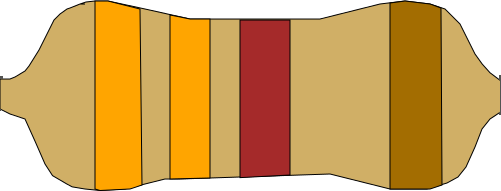
\includegraphics[angle=90, origin=c,width=1.75mm]{./images/resistor-220.png}};
            \node[] at (-.13, 1.43) {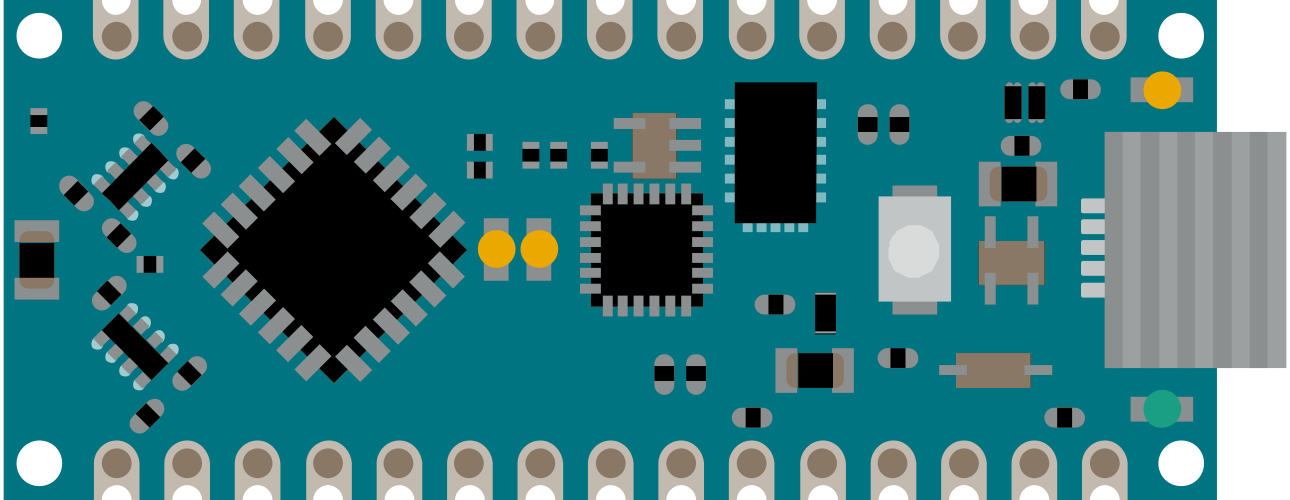
\includegraphics[angle=90, origin=c, width=3.38em]{./images/nano.png}};

            %% breadboard background
            \begin{scope}[on background layer]
                \node[] at (0, 0) {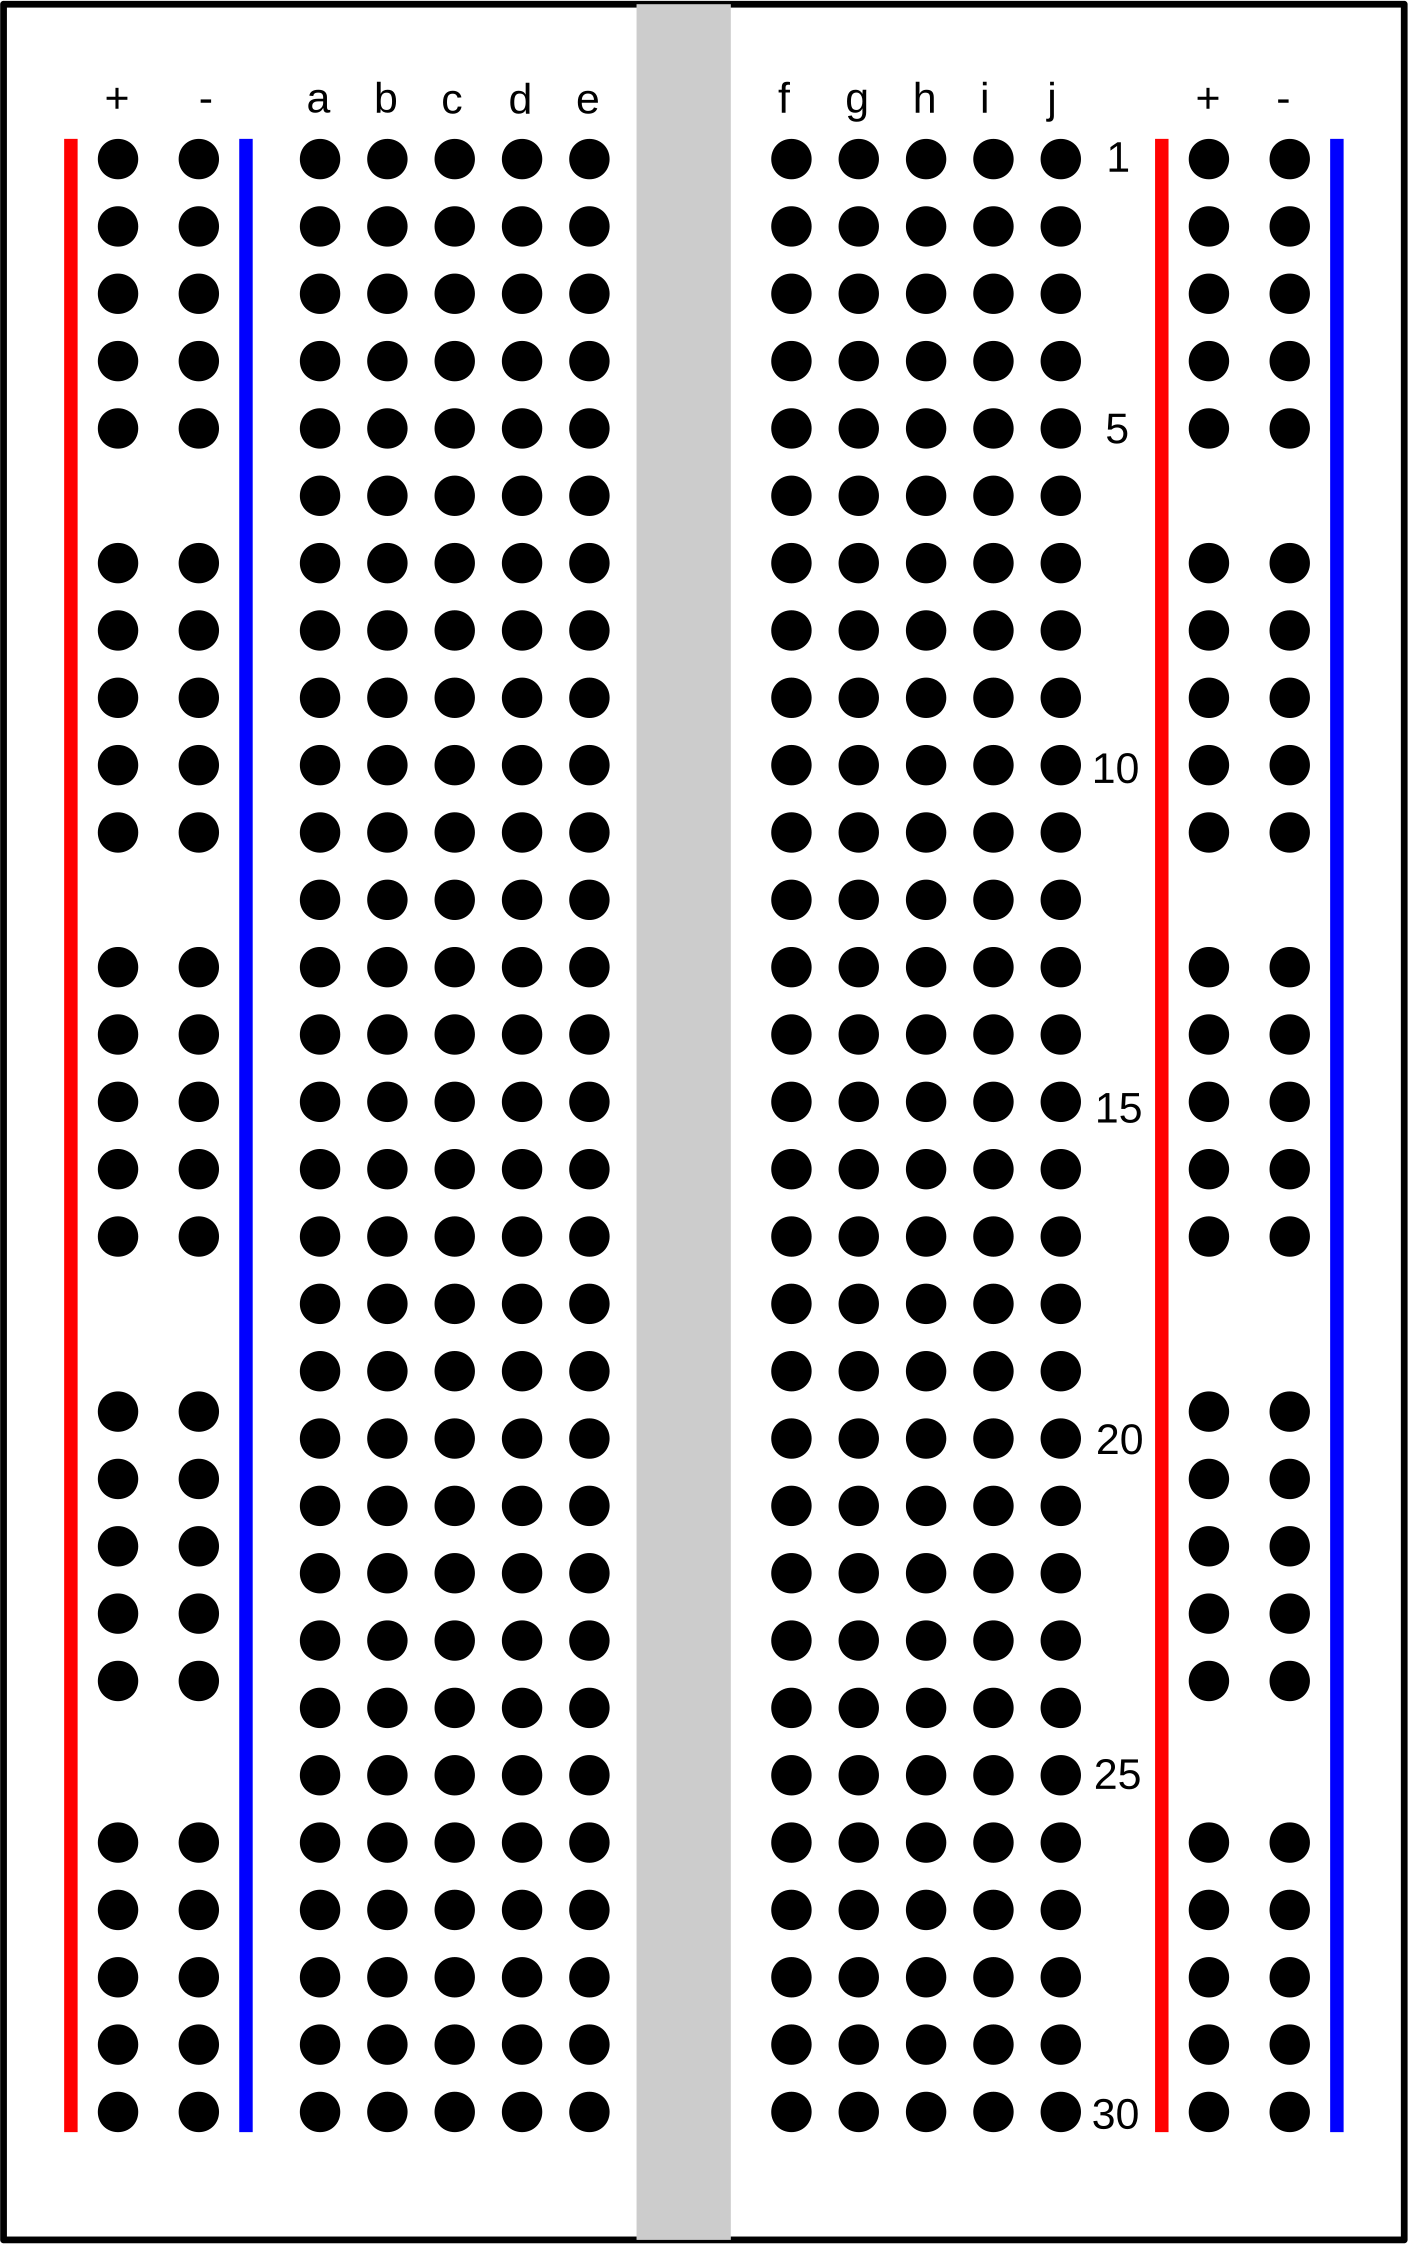
\includegraphics[width=10em]{./images/breadboard.png}};
            \end{scope}

        \end{tikzpicture}
    } 

    & \qrcode[hyperlink, height=.31\textwidth]{https://github.com/dsbrennan/mac-233-arduino-labs/blob/main/lab-2-led/lab-2-led.ino}
    \\

    & Documentation \\

    & \qrcode[hyperlink, height=.31\textwidth]{https://github.com/dsbrennan/mac-233-arduino-labs/blob/main/lab-2-led/docs/lab-2-led.pdf}\\
    
\end{tabularx}
\vspace{1em}

\subsection*{FAQ's}
\subsubsection*{Resistor issues}
If the students are unable to find which resistor is the $220\Omega$ resistor, there is a help article on blackboard under section 4a called `Reading Resistor Values'.\\
\noindent
The other issue around resistors could be students wiring the resistor in as parallel instead of series.

%%%%%%%%%%%%%%%%%%
%% Lab 3: Servo %%
%%%%%%%%%%%%%%%%%%

\section*{Lab 3: Servo}

\begin{tabularx}{\textwidth}{l@{\hspace{1em}}|@{\hspace{1em}}l}

    \hspace{0.8em}Wiring Diagram & Source Code \\

    \multirow{3}{*}[6.5em]{
        \begin{tikzpicture}[
            scale=1.75, transform shape,
            wire/.style={line width=.8mm},
            jumper/.style={draw=LimeGreen},
        ]

            %% mask out breadboard
            \filldraw[fill=white, draw=white] (0.54, -1.9) rectangle (1.04, -1.5);

            %% cables
            \draw[wire, jumper] (0.69, -1.75) -- (.607,-1.5) -- (.607, 0.604);
            \draw[wire, jumper] (0.792, -1.75) -- (.792, -0.49) to[out=130, in=50] (.42, -0.49) -- (-.87, -0.49) -- (-.87, 0.604);
            \draw[wire, jumper] (0.89, -1.75) -- (.975,-1.5) -- (.975, 2.08);

            %% components
            \draw[wire, draw=brown] (0.69,-2.32) -- (0.69, -1.75);
            \draw[wire, draw=red] (0.79,-2.32) -- (0.79, -1.75);
            \draw[wire, draw=orange] (0.89,-2.32) -- (0.89, -1.75);
            \filldraw[fill=black] (0.6, -1.8) rectangle (0.98, -1.6);
            \filldraw[fill=blue, draw=black] (-.15, -2.76) rectangle (1.05, -2.27);
            \filldraw[fill=white] (0.2,-2.51) circle (2mm);
            \node[] at (-.13, 1.43) {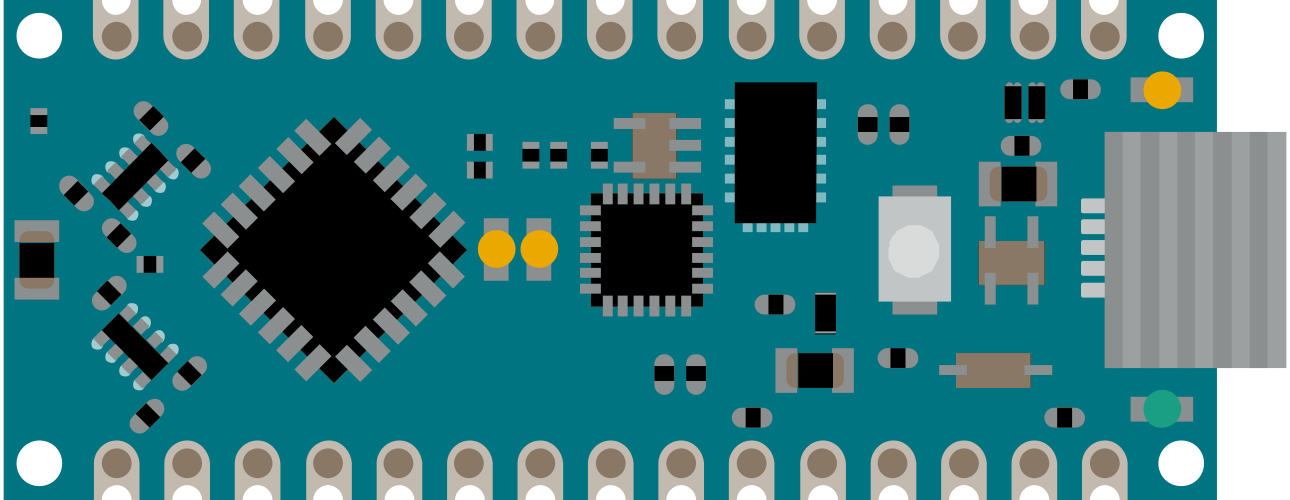
\includegraphics[angle=90, origin=c, width=3.38em]{./images/nano.png}};

            %% breadboard background
            \begin{scope}[on background layer]
                \node[] at (0, 0) {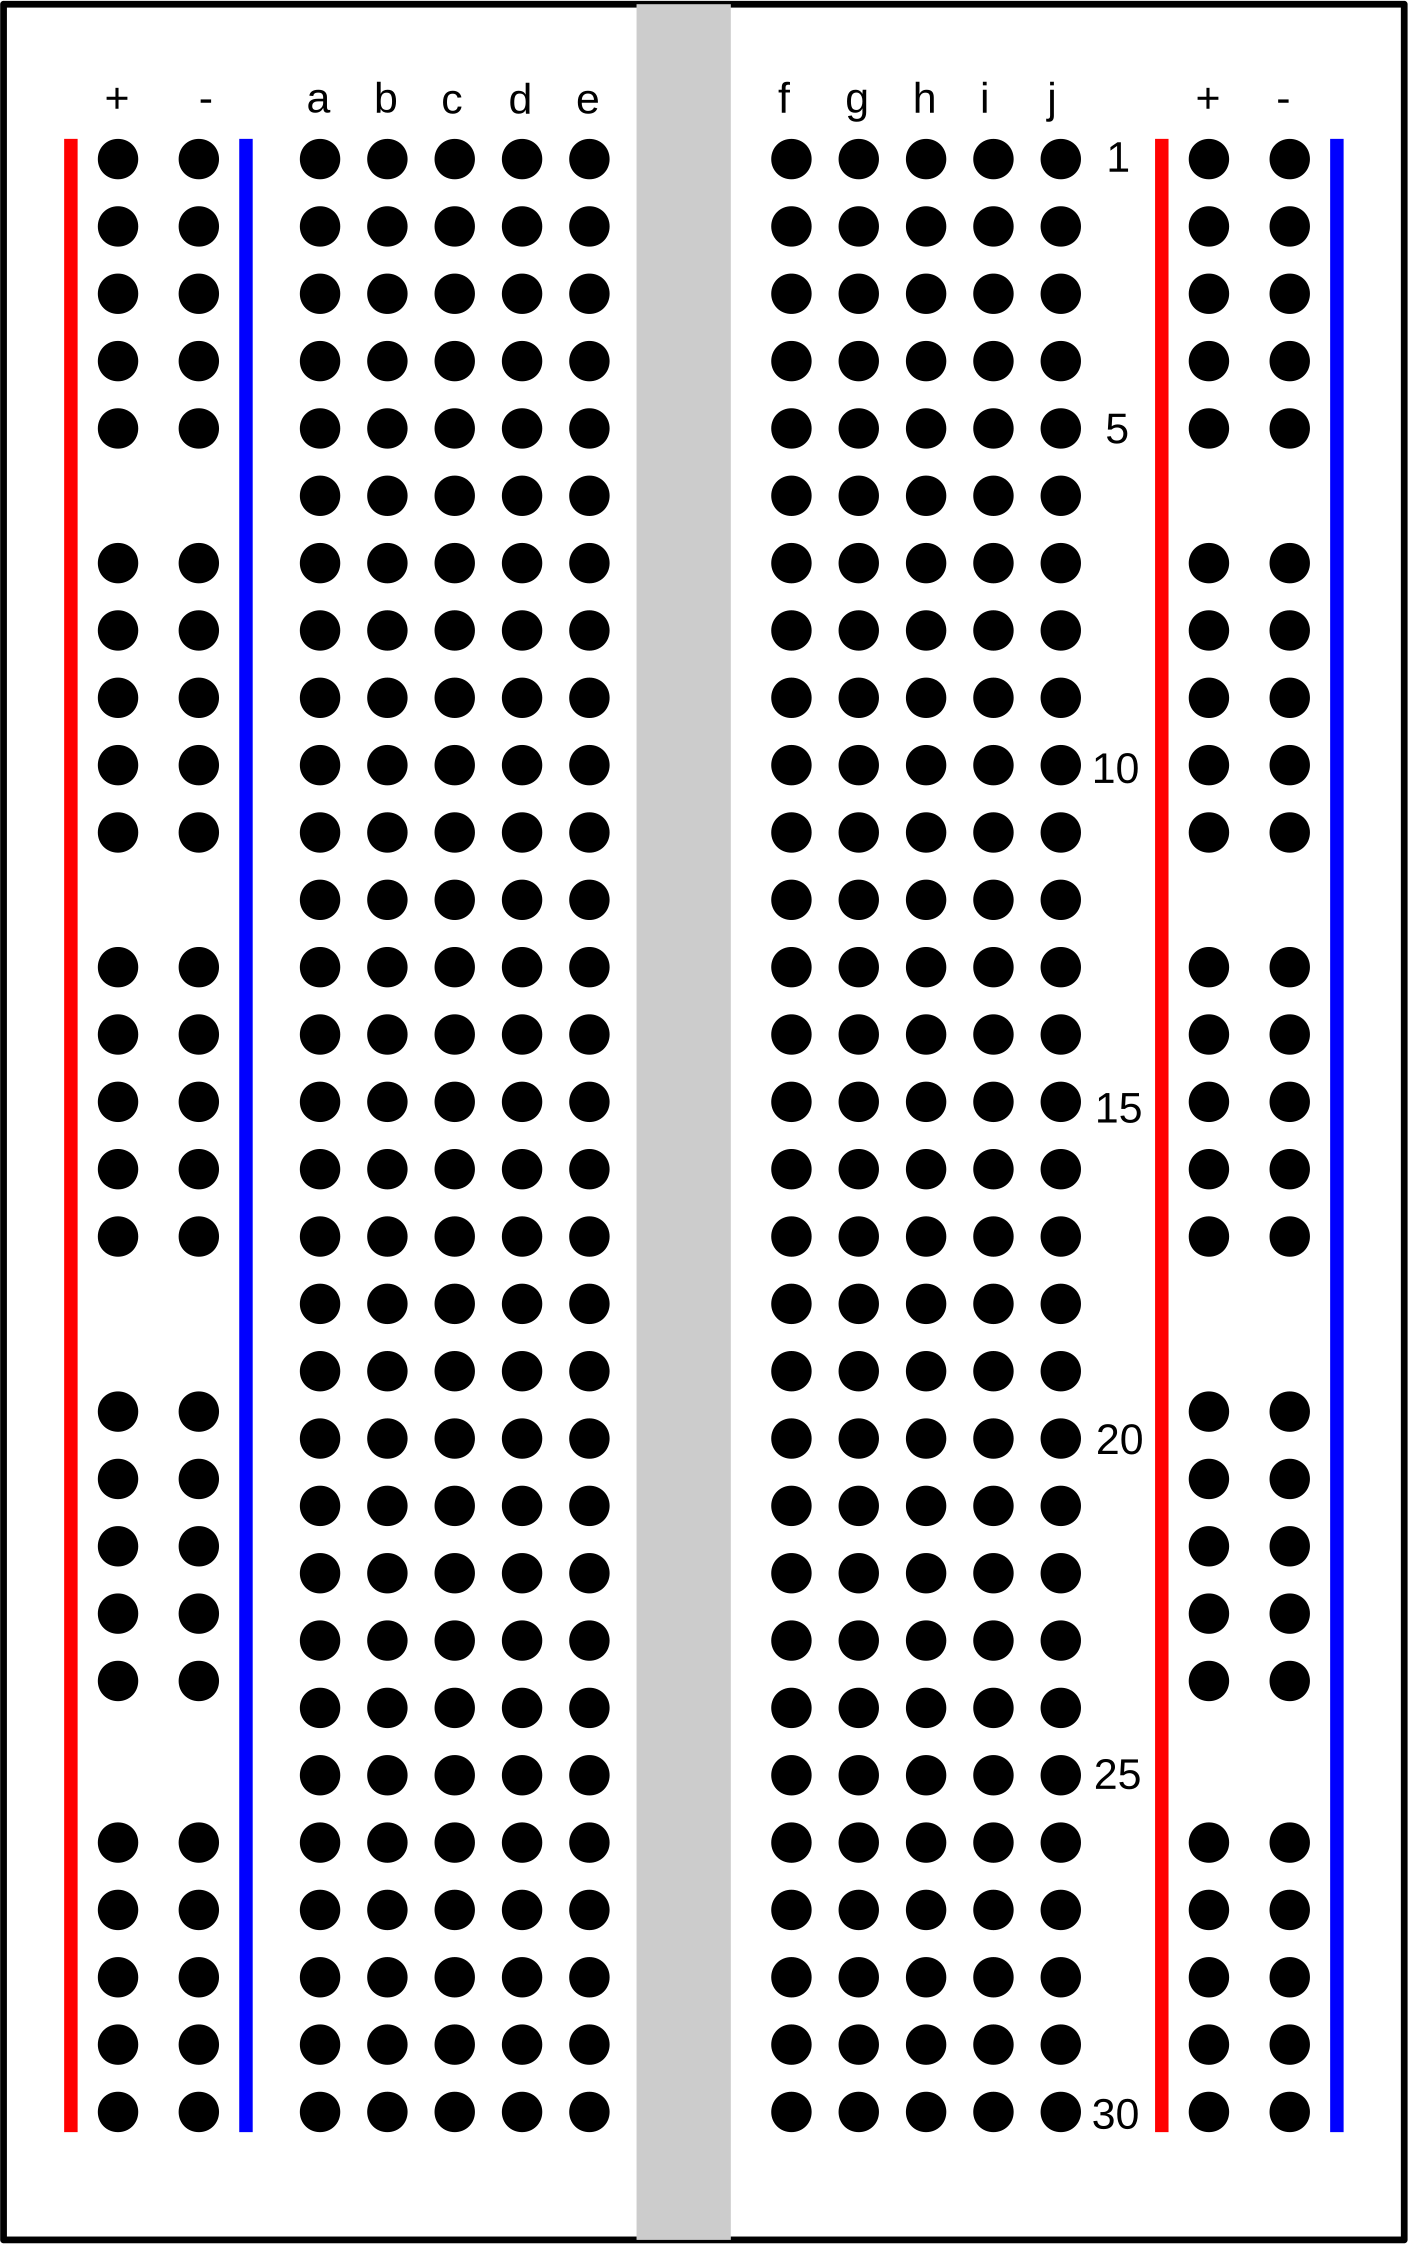
\includegraphics[width=10em]{./images/breadboard.png}};
            \end{scope}

        \end{tikzpicture}
    } 

    & \qrcode[hyperlink, height=.31\textwidth]{https://github.com/dsbrennan/mac-233-arduino-labs/blob/main/lab-3-servo/lab-3-servo.ino}
    \\

    & Documentation \\

    & \qrcode[hyperlink, height=.31\textwidth]{https://github.com/dsbrennan/mac-233-arduino-labs/blob/main/lab-3-servo/docs/lab-3-servo.pdf}\\
    
\end{tabularx}

\subsection*{FAQ's}
Coming Soon

%%%%%%%%%%%%%%%%%%%%%%%%
%% Lab 4: Hall Effect %%
%%%%%%%%%%%%%%%%%%%%%%%%

\section*{Lab 4: Hall Effect Sensors}

\begin{tabularx}{\textwidth}{l@{\hspace{1em}}|@{\hspace{1em}}l}

    \hspace{0.8em}Wiring Diagram & Source Code \\

    \multirow{3}{*}[6.5em]{
        \begin{tikzpicture}[
            scale=1.75, transform shape,
            wire/.style={line width=.8mm},
            leg/.style={draw=DimGray},
            jumper/.style={draw=LimeGreen},
        ]

            %% mask out breadboard
            \filldraw[fill=white, draw=white] (-.62, -1.49) rectangle (-.44, -0.98);

            %% legs 5 per span y = 0.188, per span x = 0.183
            \draw[wire, leg] (.975,-0.515) -- (.975, 1.16); %220 resistor
            \draw[wire, leg] (.792,-1.61) -- (.792, -0.49);%led
            \draw[wire, leg] (-.495,-1.61) -- (-.495, -0.86);%hall effect
            \draw[wire, leg] (-.69,-1.23) -- (-.59, -1.23);%hall effect
            \draw[wire, leg] (-.865,-1.61) -- (-.865, -0.86);%10k resistor

            %% cables
            \draw[wire, jumper] (.607,-1.61) -- (.607, 0.604);
            \draw[wire, jumper] (-1.05,-1.244) -- (-1.05, 0.238);
            \draw[wire, jumper] (-.31,-0.88) -- (-.31,-0.32) -- (-.865,-0.32) -- (-.865, 0.604);
            \draw[wire, jumper] (-.31,-1.61) -- (.422,-1.61) -- (.422,-0.307) to[out=50, in=130] (.792,-0.307) -- (.792, 0.792);

            %% components
            \node[] at (-.865, -1.23) {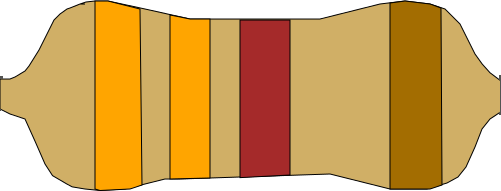
\includegraphics[angle=90, origin=c,width=1.75mm]{./images/resistor-10k.png}}; %10k resistor
            \fill[fill=red] (-.44,-1.44) -- (-.44, -1.04) -- (-.54, -1.04) -- (-.59, -1.14) -- (-.59, -1.34) -- (-.54, -1.44) -- cycle; %hall effect
            \filldraw[fill=red, draw=black] (.79,-1.05) circle (1.25mm); %led
            \node[] at (.975, 0.323) {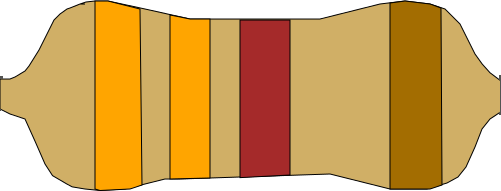
\includegraphics[angle=90, origin=c,width=1.75mm]{./images/resistor-220.png}}; %220 resistor
            \node[] at (-.13, 1.43) {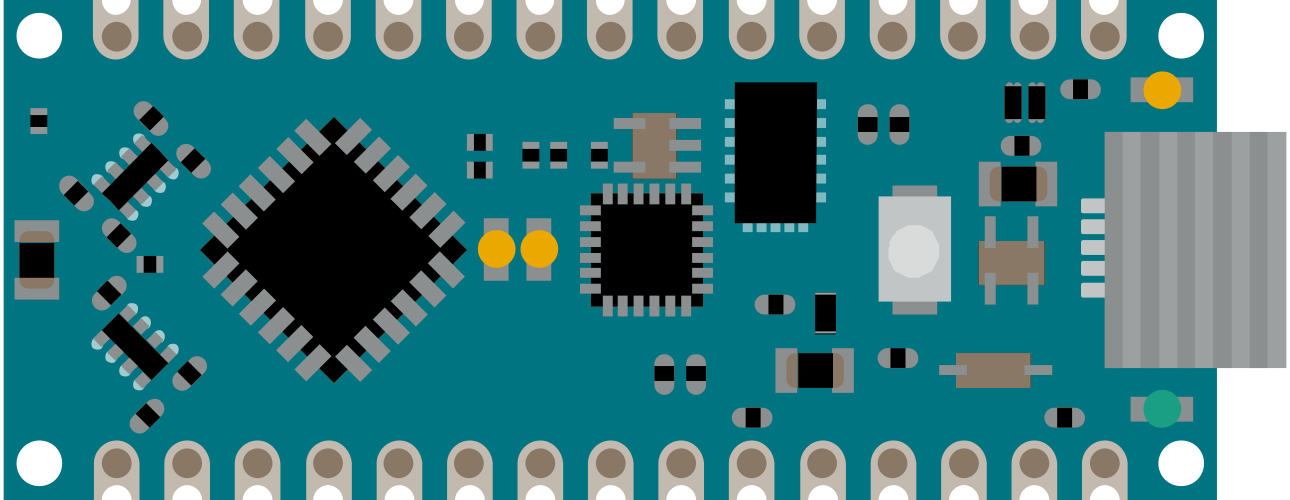
\includegraphics[angle=90, origin=c, width=3.38em]{./images/nano.png}}; %nano

            %% breadboard background
            \begin{scope}[on background layer]
                \node[] at (0, 0) {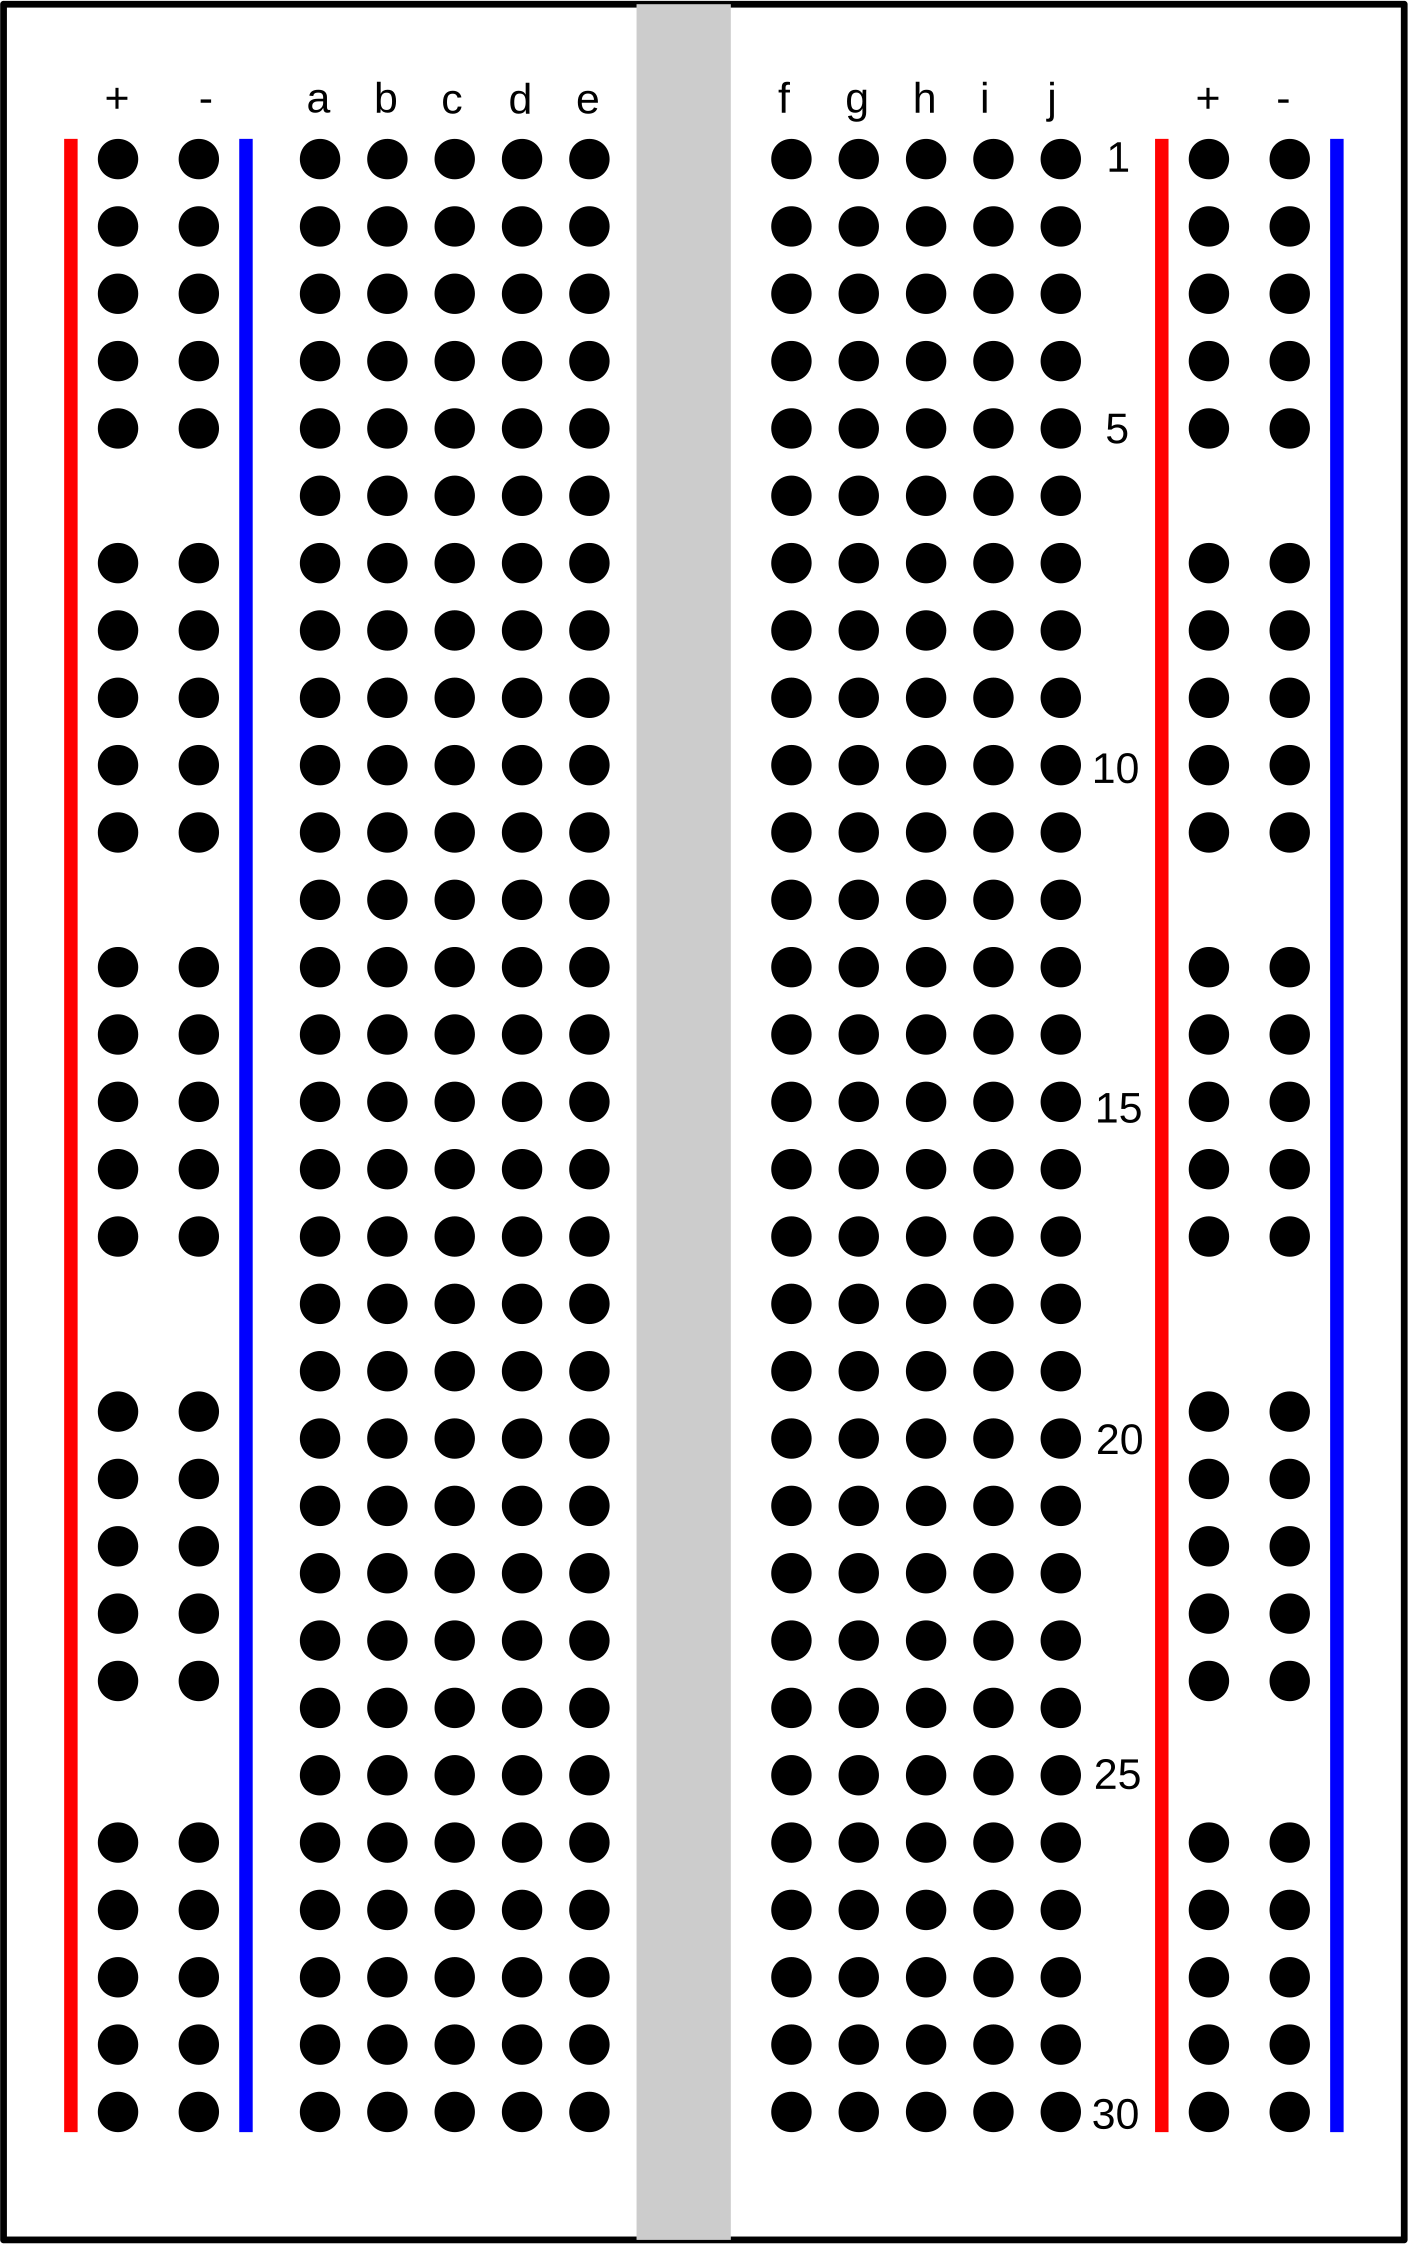
\includegraphics[width=10em]{./images/breadboard.png}};
            \end{scope}

        \end{tikzpicture}
    } 

    & \qrcode[hyperlink, height=.31\textwidth]{https://github.com/dsbrennan/mac-233-arduino-labs/blob/main/lab-4-hall-effect-sensor/lab-4-hall-effect-sensor.ino}
    \\

    & Documentation \\

    & \qrcode[hyperlink, height=.31\textwidth]{https://github.com/dsbrennan/mac-233-arduino-labs/blob/main/lab-4-hall-effect-sensor/docs/lab-4-hall-effect-sensor.pdf}\\
    
\end{tabularx}

\subsection*{FAQ's}
Coming Soon


%%%%%%%%%%%%%%%%%%%%%%%%%%%
%% Lab 5: Control System %%
%%%%%%%%%%%%%%%%%%%%%%%%%%%

% \section*{Lab 5: Control System}

% \begin{tabularx}{\textwidth}{l@{\hspace{1em}}|@{\hspace{1em}}l}

%     Wiring Diagram & Source Code \\

%     \multirow{3}{*}[6.5em]{

%     } 

%     & \qrcode[hyperlink, height=.31\textwidth]{https://github.com/dsbrennan/mac-233-arduino-labs/blob/main/lab-5-control-system/lab-5-control-system.ino}
%     \\

%     & Documentation \\

%     & \qrcode[hyperlink, height=.31\textwidth]{https://github.com/dsbrennan/mac-233-arduino-labs/blob/main/lab-5-control-system/docs/lab-5-control-system.pdf}\\
    
% \end{tabularx}

% \subsection*{FAQ's}


\section*{Images}
Original images for the wiring is taken from:
\begin{itemize}
    \item Breadboard (\url{https://freesvg.org/breadboard})
    \item Resistor (\url{https://freesvg.org/resistor-330-ohm})
\end{itemize}

\end{document}